\section{Introduction}

\begin{figure}
    \centering
    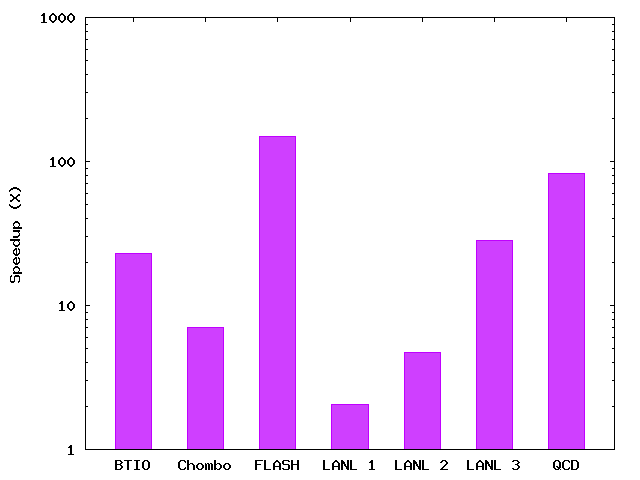
\includegraphics[width=0.4\textwidth]{data/summary/page1.eps}
    \mycaption{fig-page1}{Summary of our results.}{
        This graph summarizes our results which will be
        explained in detail in Section~\ref{eval}.  
        The key observation here is that our technique
        has improved checkpoint bandwidths for all seven
        studied benchmarks and applications by up to
        several orders of magnitude.  
        \vspace{1.0cm}
    }
\end{figure}


\scribble{Need to define "its class" --Milo}
% computers are large, they have failures
In June 2008, Los Alamos National Labs (LANL), in partnership with IBM, broke
the petaflop barrier and claimed the top spot on the Top 500 list~\cite{top500}
with the Roadrunner supercomputer~\cite{roadrunner}.  Due to its unique hybrid
architecture, Roadrunner has only 3060 nodes, which is a relatively small
number for a supercomputer of its class.  Unfortunately, even at this size,
component failures are frequent.  For large parallel simulations at
LANL, and other High Performance Computing (HPC) sites, which can run for
several months, restarting a calculation from the beginning is not viable,
since the mean time to interrupt for today's supercomputers is measured in days
or hours and not months~\cite{google-failure,schroeder-failure}.  

\begin{figure*}[tb]
  \centering
    \fbox{
        \subfloat[N-N]{\label{fig:nn}
            \includegraphics[width=0.25\textwidth]{figs/nn-arrows.eps}}
    }
    \fbox{
        \subfloat[N-1 segmented]{\label{fig:n1segmented}
           \includegraphics[width=0.25\textwidth]{figs/n1nonstrided-arrows.eps}}
    }
    \fbox{
        \subfloat[N-1 strided]{\label{fig:n1strided}
            \includegraphics[width=0.25\textwidth]{figs/n1strided-arrows.eps}}
    }
    \mycaption{fig-patterns}{Common Checkpointing Patterns.}{
This figure shows the three basic checkpoint patterns: from left to right, N-N,
N-1 segmented, and N-1 strided.  In each pattern, the parallel application is
the same, consisting of six processes spread across three compute nodes each of
which has three blocks of state to checkpoint.  The difference in the three
patterns is how the application state is logically organized on disk.  In the
N-N pattern, each process saves its state to a unique file.  N-1 segmented is
simply the concatenation of the multiple N-N files into a single file.
Finally, N-1 strided, which also uses a single file as does N-1 segmented, has
a region for each block instead of a region for each process.  From a parallel
file system perspective, N-1 strided is the most challenging pattern as it is
the most likely to cause small, interspersed, and unaligned writes.  Note that
previous work~\cite{hedges-lunatic} refers to N-N as \Term{file per process}
and N-1 as \Term{shared file} but shares our segmented and strided terminology.
}
\end{figure*}


% checkpoint is defense against failure, drives parallel file systems, is
% challengin
Typically these applications protect themselves against failure by periodically
\Term{checkpointing} their progress by saving the state of the application to
persistent storage. After a failure the application can then restart from the most recent 
checkpoint.  Due to the difficulty of reconstructing a consistent
image from multiple asynchronous checkpoints~\cite{lamport1978}, HPC
applications checkpoint synchronously (\ie\ following a barrier).  Synchronous
checkpointing, however, does not eliminate the complexity; it merely shifts it to
the parallel file system which now must coordinate simultaneous access from
thousands of compute nodes.  Even using optimal checkpoint frequencies~\cite{daly-optimal}, 
checkpointing has become the driving workload for
parallel file systems and the challenge it imposes grows with each successively
larger supercomputer~\cite{pcl:99:me,schroeder2007}.  The difficulty of this
challenge can vary greatly depending on the particular pattern of checkpointing
chosen by the application. 
In this paper, we describe different checkpointing patterns, and show how some
result in very poor storage performance on three of the major HPC
parallel file systems: PanFS, GPFS, and Lustre.  

We then posit that an
interposition layer inserted into the existing storage stack can rearrange this
problematic access pattern to achieve much better performance from the
\upfs.  To test this hypothesis, we have developed \plfs, a Parallel
Log-structured File System, one such interposition layer.  We present measurements using \plfs\ on several synthetic benchmarks and real applications at multiple HPC supercomputing centers.  The
results confirm our hypothesis: writing to the \upfs\ through
\plfs\ improves checkpoint bandwidth for all tested applications and
benchmarks and on all three studied parallel file systems; in some cases,
bandwidth is raised by several orders of magnitude.

As we shall discuss, and is summarized in Figure~\ref{fig-page1}, \plfs\ is
already showing very large speed ups for widely used HPC benchmarks and
important real HPC codes, and at extreme scale.  \plfs\ works on unmodified
applications as an optional mount point on the compute nodes and is designed to
augment, and not replace, an existing \upfs.  \plfs\ consists of three thousand
lines of code and is publically available at
http://sourceforge.net/projects/plfs.

% the stupid mandatory list of the rest of the paper
The rest of the paper is organized as follows.  We present more detailed background and
motivation in Section~\ref{motivation}, describe our design in
Section~\ref{arch} and our evaluation in Section~\ref{eval}.  We present
related work in Section~\ref{related}, current status and future work in
Section~\ref{future}, and finally we conclude in Section~\ref{conclude}.

